%!TEX TS-program = pdflatex
%!TEX root = tesi.tex
%!TEX encoding = UTF-8 Unicode

%\begin{figure}[ht] % TODO remove me
%  \begin{center}
%    \begin{tabular}{ccc}
%
%  \begin{subfigure}{.3\linewidth}
%    \centering\includegraphics[width=\textwidth]{example-image}
%    \caption{}
%  \end{subfigure} &
%
%    \end{tabular}
%    \caption{Alcune carcasse Conformi}
%    \label{fig:esempi_conformi}
%  \end{center}
%\end{figure}



\chapter{Gli Autoencoder}

Breve intuizione sugli AE
\todo[inline]{TODO recap capitolo}

\section{La Struttura di un Autoencoder}
Un \textit{Autoencoder}(AE) è un particolare tipo di rete neurale.
Può essere diviso in due componenti: il primo viene chiamato \textit{encoder}, mentre il secondo prende il nome di \textit{decoder}.
Lo scopo dell'\textit{encoder} è codificare il dato in ingresso in una versione compressa.
Sia $n$ la dimensionalità dell'\textit{input}.
Quando il dato raggiunge il collo di bottiglia dell'AE, ovvero la parte centrale della rete, ha raggiunto il livello di massima compressione, sia $m$ la sua nuova dimensionalità con $m<n$.
Lo spazio $m$-dimensionale in cui l'informazione è stata mappata viene chiamato spazio latente o spazio nascosto.
Ora il dato può essere decompresso dal \textit{decoder}, in questo modo verrà riportato alle sue dimensioni originali, cioè mappato nello spazio $n$-dimensionale di partenza.

Visto dall'esterno, il compito di un \textit{autoencoder} è quello di ritornare un valore il più simile al dato in ingresso.
Durante l'allenamento, fissato $m$ con un valore che dipende dalla forma della rete, si vuole trovare il miglior spazio latente possibile.
Dove con migliore si intende quello spazio di cardinalità $m$ che permette di mantenere tutte le informazioni caratterizzanti dell'input.
Riformulando quanto detto: un'\textit{autoencoder} può essere visto come una funzione $f$ rassomigliante la funzione identità, ma al cui intero c'è un vincolo tale da rendere il compito di restituzione dell'\textit{input} non banale.

Come viene spiegato da Andrew Ng in \cite{ng_sparse_ae}, gli \textit{autoencoder} fanno parte degli algoritmi di apprendimento non supervisionato.
Cioè di quella classe di algoritmi, in contrapposizione a quelli ad apprendimento supervisionato, che non ha bisogno di dati etichettati; anzi vengono usati proprio per trovare nuovi pattern e correlazioni tra gli elementi del \textit{dataset}.
Come gli algoritmi \textit{K-Means} e \textit{DBSCAN}, entrambi di \textit{clustering}, permettono di raggruppare nuvole di punti con caratteristiche simili. % TODO citare?
%I gruppi così creati possono far risaltare degli andamenti dei dati 
Un AE è non supervisionato perché, a priori, non conosciamo la forma che verrà data allo spazio latente. % TODO espandere?

Gli \textit{autoencoder} più semplici sono composti da due strati densamente connessi di neuroni: il primo funge da \textit{encoder} ed ha un numero di unità pari alla dimensione dello spazio latente; il secondo ha tante unità quanto la dimensione dell'\textit{input}, quindi funge da \textit{decoder}.
L'architettura appena descritta può essere osservata in figura~\ref{fig:semplice_ae}, notare la tipica forma a clessidra.

\begin{figure}[ht] % TODO rifare con tikz
  \begin{center}
    %\centering\includegraphics[width=.4\textwidth]{example-image}
    \centering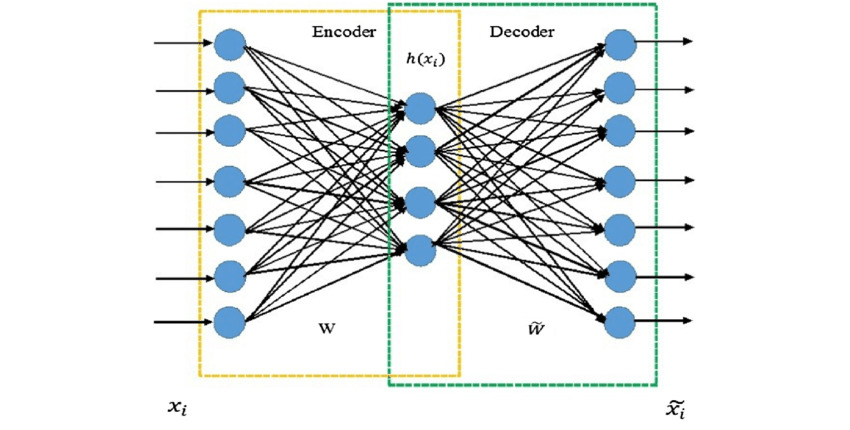
\includegraphics[width=\textwidth]{simple_ae}
  \end{center}
  \caption{Architettura di un semplice \textit{autoencoder}}
  \label{fig:semplice_ae}
\end{figure}

Facendo sempre rifermento a \cite{ng_sparse_ae}, un neurone è un'unità computazionale che prende in \textit{input} un vettore $x$ di elementi $x_i$ con $i=1,2,3,\dots,n$ e che ritorna $h_{W,b}(x) = f(W^Tx) = f(\sum_{i=1}^{n} W_i x_i + b)$.
Dove $h_{W,b}(x)$ è un generatore di ipotesi non-lineare, con parametri $W$ e $b$ che possono adattarsi al \textit{dataset}.
I pesi del neurone vengono salvati in $W$, vettore con tanti elementi quanti quelli di $x$.
%bias = pregiudizio
Il valore $b$ viene detto \textit{bias} è una quantità che verrà sempre sommata al risultato del prodotto riga per colonna tra $W$ e $x$.
% TODO fare figura a cui posso riferirmi per spiegare dove sono messi i pesi
La funzione $f$ è chiamata funzione di attivazione.
Come funzione di attivazione viene spesso utilizzata la funzione sigmoidea:
\begin{equation*}
  f(z) = \frac{1}{1 + exp(-z)}
\end{equation*} %TODO fare plot?
Notare come $f(z)$ sia una una funzione da $\mathbb{R}$ in $[0,1]$.
Ciò risulta utile per vari motivi:
\begin{itemize}
  \item se il compito del neurone è dividere gli \textit{input} in due classi distinte, cioè $0$ e $1$, basterà verificare se $f(z)>0.5$.
    In caso affermativo l'\textit{input} verrà associato alla classe con etichetta $1$, altrimenti a $0$;
  \item un'altra motivazione è evitare che, se la rete è composta da molti strati, i valori in uscita, strato dopo strato, sempre più grandi. Con la funzione sigmoidea gli \textit{output} vengono limitati nell'intervallo $[0,1]$.
\end{itemize}

Quando uno strato della rete è composto da più neuroni, ciascuno di essi riceverà una copia di $x$ e ritornerà un \textit{output} in base ai propri $W$ e $b$.
In figura~\ref{fig:semplice_ae} si può notare come gli $x_i$ vengano distribuiti su tutti i nodi del primo strato e come il loro risultato venga a sua volta distribuito sulle altre unità.
Dato che il numero di connessioni cresce rapidamente, essendo pari a $n*m$ per ogni strato (con $n$ la dimensione del vettore in ingresso ed $m$ di quello in uscita), questi strati vengono chiamati densamente connessi o, più semplicemente, densi.

Nonostante gli Ae semplici abbiano dato ottimi risulatati cfr. AE vs PCA si è esplocratta la possibilità di aumentare il numero di strati

\begin{figure}[ht] % TODO rifare con tikz
  \begin{center}
  % https://www.researchgate.net/figure/Stacked-autoencoders-architecture_fig21_319524552
    \centering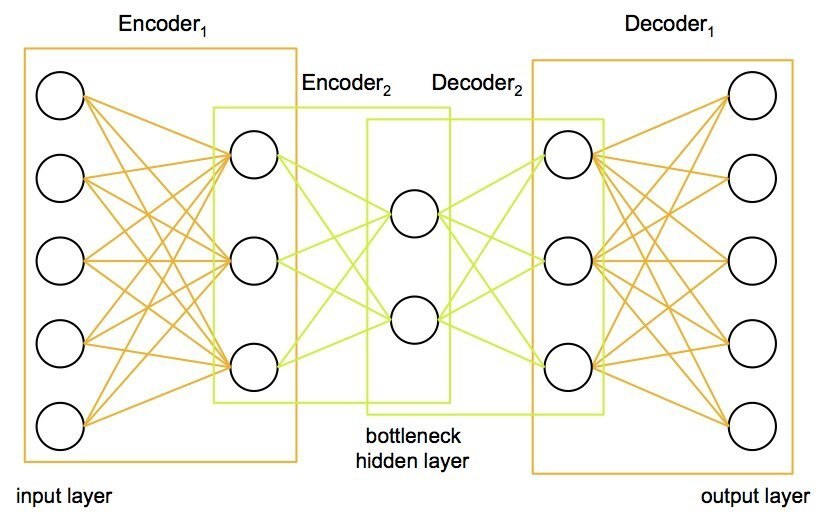
\includegraphics[width=\textwidth]{stacked_ae}
  \end{center}
  \caption{Architettura di un \textit{stacked autoencoder}}
  \label{fig:stacked_ae}
\end{figure}












\clearpage
\todo[inline]{spiegare Conv, ConvTransposed, MaxPool, Upsampling}
\clearpage
\subsection{Applicazioni principali}

\paragraph{Denoising}

\paragraph{Variational}

\paragraph{Anomaly Detection}
